%%%%%%%%%%%%%%%%%%%%%%%%%%%%%%%%%%%%%%%%%
% Beamer Presentation
% LaTeX Template
% Version 1.0 (10/11/12)
%
% This template has been downloaded from:
% http://www.LaTeXTemplates.com
%
% License:
% CC BY-NC-SA 3.0 (http://creativecommons.org/licenses/by-nc-sa/3.0/)
%
%%%%%%%%%%%%%%%%%%%%%%%%%%%%%%%%%%%%%%%%%

%----------------------------------------------------------------------------------------
%	PACKAGES AND THEMES
%----------------------------------------------------------------------------------------

\documentclass{beamer}

\mode<presentation> {

% \usetheme{Madrid}

\setbeamertemplate{navigation symbols}{} % To remove the navigation symbols from the bottom of all slides uncomment this line
}

\usepackage{graphicx} % Allows including images
\usepackage{booktabs} % Allows the use of \toprule, \midrule and \bottomrule in tables
\usepackage{bbm}
\usepackage{amssymb}
\usepackage{amsmath}
\usepackage{textpos}
% \usepackage{subfigure}
% \usepackage{cite}
\usepackage[T1]{fontenc}
\usepackage{subfig}
\usepackage{listings}
\usepackage{mathtools}

\newcommand{\p}{\text{p}}

\definecolor{gray}{rgb}{0.4,0.4,0.4}
\definecolor{darkblue}{rgb}{0.0,0.0,0.6}
\definecolor{cyan}{rgb}{0.0,0.6,0.6}

\lstset{
  basicstyle=\ttfamily,
  columns=fullflexible,
  showstringspaces=false,
  commentstyle=\color{gray}\upshape
numbers=right, 
                numberstyle=\tiny, 
                breaklines=true,
                numbersep=5pt,
                xleftmargin=.25in,
                xrightmargin=.25in
}

\lstdefinelanguage{XML}
{
  morestring=[b]",
  morestring=[s]{>}{<},
  morecomment=[s]{<?}{?>},
  stringstyle=\color{black},
  identifierstyle=\color{darkblue},
  keywordstyle=\color{cyan},
  morekeywords={xmlns,version,type}% list your attributes here
}

\DeclareMathOperator*{\argmax}{\arg\!\max}

\title[Automatic Metadata Extraction]{Automatic Metadata Extraction \\ The High Energy Physics Use Case} % The short title appears at the bottom of every slide, the full title is only on the title page

\author{Joseph Boyd} % Your name
\institute[EPFL] % Your institution as it will appear on the bottom of every slide, may be shorthand to save space
{
\'Ecole Polytechnique F\'ed\'erale de Lausanne \\ % Your institution for the title page
\medskip
\textit{joseph.boyd@epfl.ch} % Your email address
}
\date{\today} % Date, can be changed to a custom date

% \logo{
\includegraphics[height=1cm]{Figures/EPFL-logo.jpg} \ \ 
\includegraphics[height=1cm]{Figures/CERN-logo.jpg}}

\begin{document}

\begin{frame}
\titlepage % Print the title page as the first slide
\end{frame}

%------------------------------------------------

\section{Introduction}

%------------------------------------------------

\begin{frame}
\frametitle{Motivation}
\begin{itemize}
\item INSPIRE-HEP digital library at CERN contains over 1 Million documents
\item Manual curation of high energy physics (HEP) papers may be automated with machine learning techniques
\item Custom datasets and specialised features required to model HEP paper characteristics
\end{itemize}
\end{frame}

%------------------------------------------------

\begin{frame}
\frametitle{Aims}
Take existing state-of-the-art system for metadata extraction to:
\begin{itemize}
\item demonstrate a qualitative difference between HEP and general papers;
\item propose improvements to model features;
\item run experiments to confirm these improvements, and;
\item draw conclusions about what characterises good feature engineering.
\end{itemize}
\end{frame}

%------------------------------------------------

%\section{Theory}
%
%%------------------------------------------------
%
%\begin{frame}[noframenumbering]{Outline}
%\tableofcontents[currentsection, currentsubsection]
%\end{frame}
%
%%------------------------------------------------
%
%\begin{frame}
%\frametitle{Why Conditional Random Fields?}
%\begin{itemize}
%\item Transition interdependencies implies graphical structure best modelled as a structured sequence
%\item Modelling conditional distribution, $p(\textbf{y}|\textbf{x})$, sufficient for classification
%\item Exploit rich information about observations, $\textbf{x}$, without explicitly modelling the underlying probability distribution
%\item Classifying metadata may greatly benefit from modelling rich text features (punctuation, font size, layout ...)
%\end{itemize}
%\end{frame}
%
%%------------------------------------------------
%
%\begin{frame}
%\frametitle{Mathematical Formulation}
%
%A CRF factorises in the following as,
%
%$$
%\p(\textbf{y}|\textbf{x}) = \frac{\p(\textbf{x}, \textbf{y})}{\sum_{y'}{\p(\textbf{x}, \textbf{y}')}} = \frac{1}{Z(\mathbf{x})}\exp \Bigg\{\sum_k{
%\lambda_{k}F_{k}(y_t, y_{t-1}, x_t)
%}\Bigg\},
%$$
%
%
%
%\begin{itemize}
%\item  $Z(\mathbf{x}) = \sum_{y'}\exp \Big\{\sum_k{\lambda_{ij}F_{k}(y'_t, y'_{t-1}, x_t)}\Big\}$, known as the parition function.
%\item $F_k(\mathbf{x}, y) = \sum_t^T f_k(\mathbf{x}, y)$, where $f_k$ is a function expressing a feature.
%\item It is in choosing the form of the functions, $f(\cdot)$, explicitly that we perform feature engineering.
%\end{itemize}
%
%\end{frame}
%
%%------------------------------------------------
%
%\begin{frame}
%\frametitle{Solution Approach}
%\begin{itemize}
%\item Formulate convex function, maximum log likelihood estimator, $l(\Lambda)$, where $\Lambda = \{\lambda_k\}_{k=1}^K$.
%\item Train (determine $\Lambda$) with gradient ascent technique, L-BFGS. Each iteration, $I$, requires forward-backward algorithm to compute $Z(\mathbf{x^{(n)}})$ for each of $N$ samples -- $\mathcal{O}(INT|S|^2)$.
%\item Prediction with Viterbi algorithm -- $\mathcal{O}(T|S|^2)$.
%\end{itemize}
%\end{frame}
%
%%------------------------------------------------

\section{Automatic Metadata Extraction}

%------------------------------------------------

\begin{frame}[noframenumbering]{Outline}
\tableofcontents[currentsection, currentsubsection]
\end{frame}

%------------------------------------------------

\begin{frame}
\frametitle{Metadata Extraction}
\begin{itemize}
\item \emph{Metadata} refers to content useful to the bibliographpic identification of the document
\item \emph{Extraction} refers to the classification of metadata within the document text
\item Several automatic approaches exist: stylistic analysis, knowledge-base, machine learning (CRFs, HMMs, SVMs) ...
\end{itemize}
\end{frame}

%------------------------------------------------

\begin{frame}
\frametitle{Metadata Extraction (Illustration)}
\begin{figure}[h]
\center
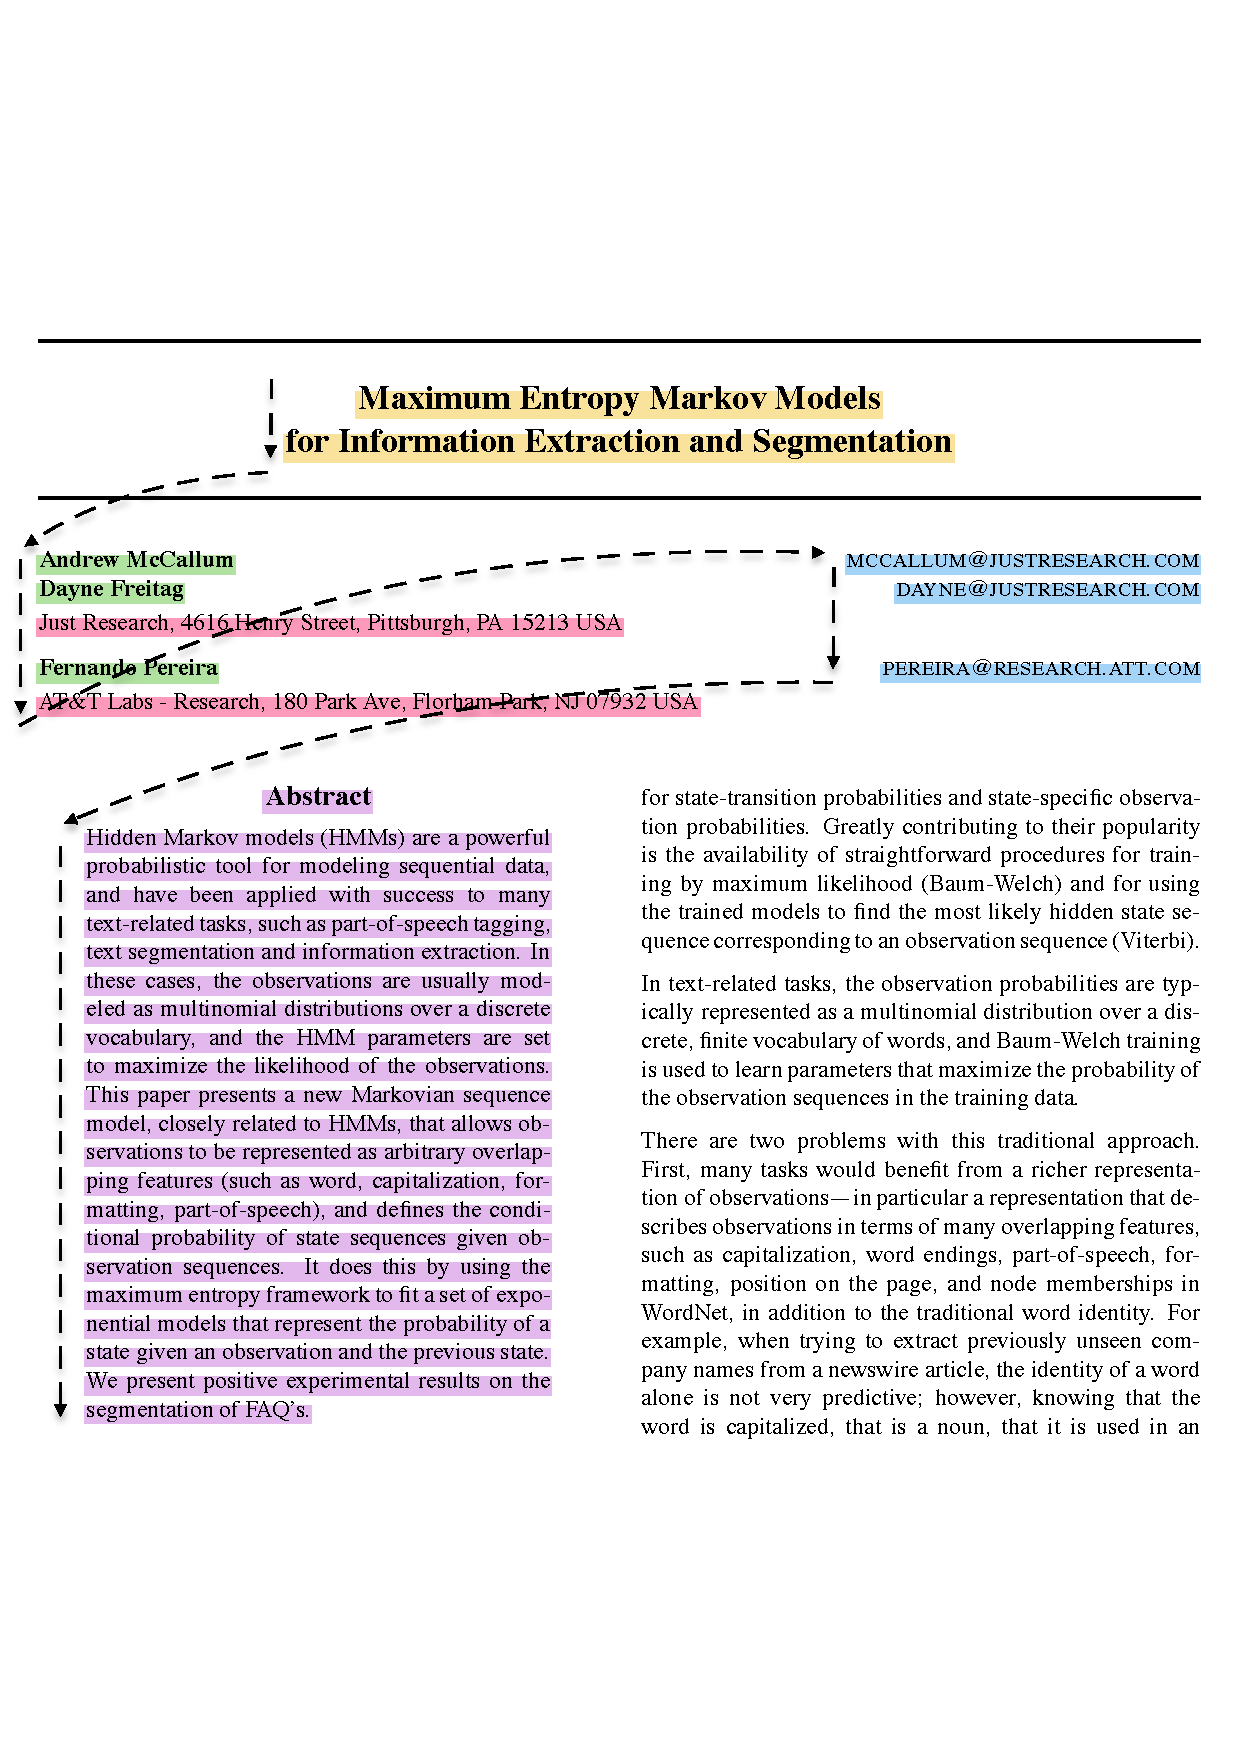
\includegraphics[width=3in]{Figures/extraction.pdf}
\caption{Tagging of a document header section.}
\end{figure}
\end{frame}

%------------------------------------------------

\begin{frame}
\frametitle{Why Conditional Random Fields?}
\begin{itemize}
\item Transition interdependencies implies graphical structure best modelled as a structured sequence
\item Modelling conditional distribution, $p(\textbf{y}|\textbf{x})$, sufficient for classification
\item Exploit rich information about observations, $\textbf{x}$, without explicitly modelling the underlying probability distribution
\item Classifying metadata may greatly benefit from modelling rich text features (punctuation, font size, layout ...)
\end{itemize}
\end{frame}

%------------------------------------------------

\begin{frame}
\frametitle{GROBID}
\begin{itemize}
\item Selected according to performance in study comparing AME systems \cite{
lipinski2013evaluation}
\item Open source Java-based tool developed at INRIA, France
\item Manages \emph{cascade} of CRF models for annotating papers in progressively finer detail
\item Uses C++ library \emph{Wapiti} for back-end calculations (model training, prediction)
\end{itemize}
\end{frame}

%------------------------------------------------

\begin{frame}
\frametitle{GROBID - CRF Cascade}
\begin{figure}[h]
\center
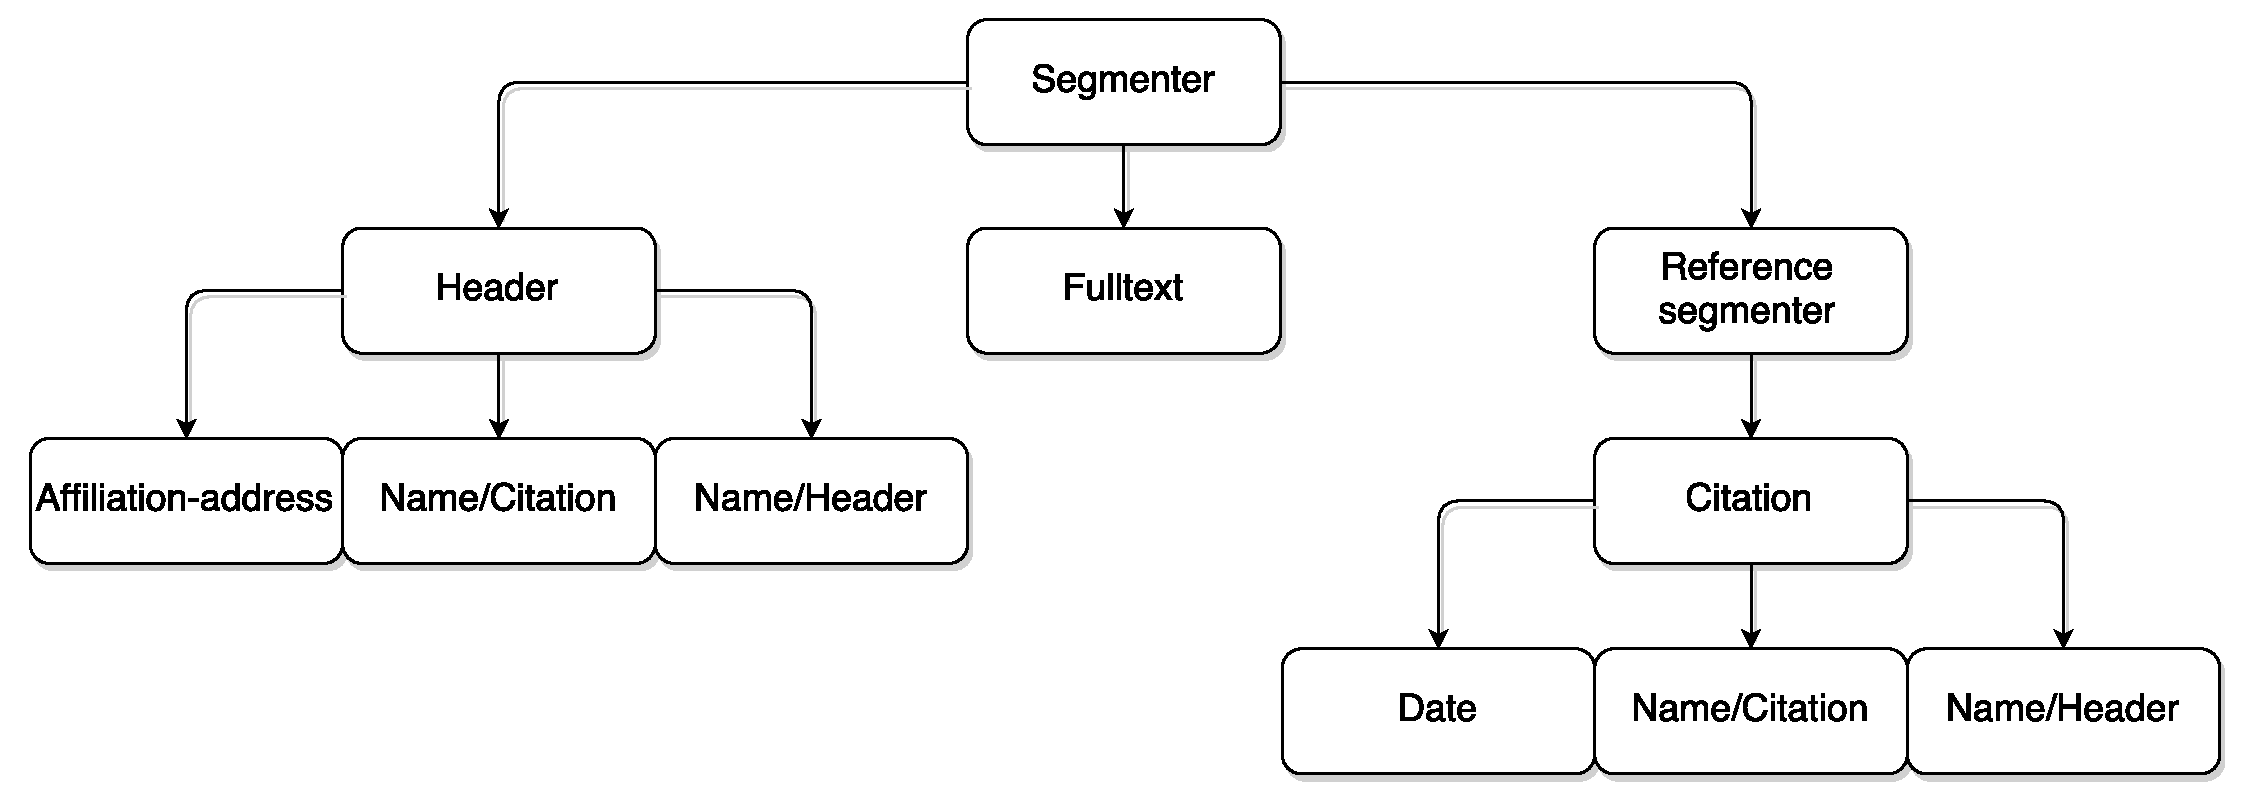
\includegraphics[width=\textwidth]{Figures/cascade.pdf}
\caption{Cascade of models used by Grobid}
\end{figure}
\end{frame}

%------------------------------------------------

\section{Data and Features}

%------------------------------------------------

\begin{frame}[noframenumbering]{Outline}
\tableofcontents[currentsection, currentsubsection]
\end{frame}

%------------------------------------------------

\begin{frame}
\frametitle{HEP Paper Characteristics (i)}
\begin{figure}[h]
\center

\includegraphics[width=3in]{Figures/collaboration.pdf}
\caption{Collaboration field in header section.}
\end{figure}
\end{frame}

%------------------------------------------------

\begin{frame}
\frametitle{HEP Paper Characteristics (ii)}
\begin{figure}[h]
\center
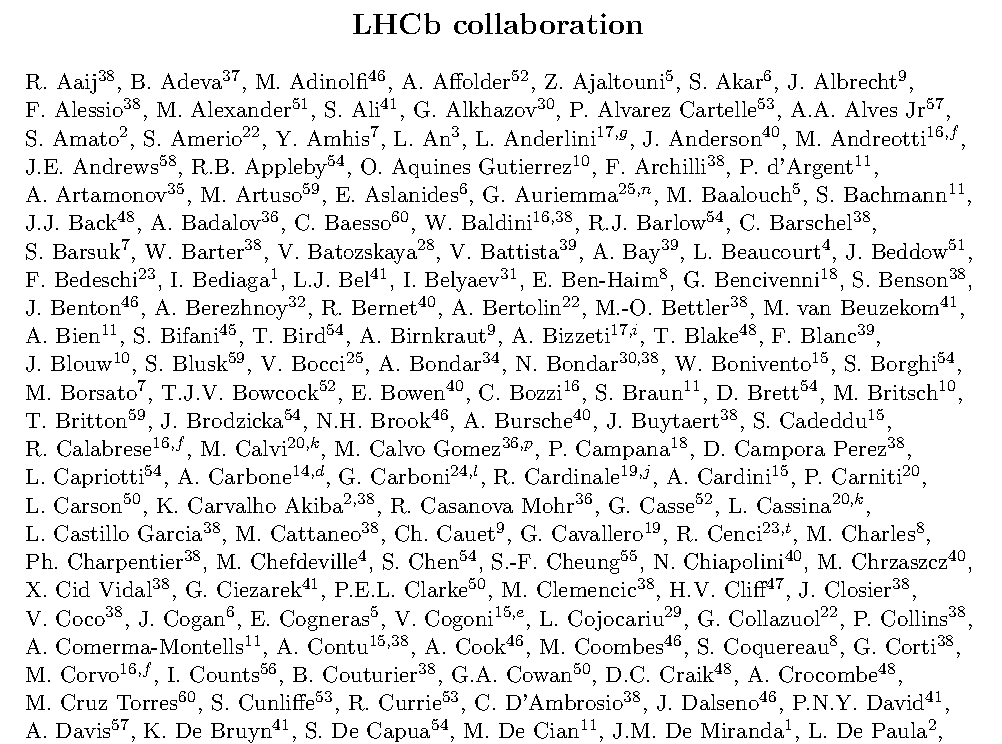
\includegraphics[width=3in]{Figures/authors.pdf}
\caption{Collaboration author list.}
\end{figure}
\end{frame}

%------------------------------------------------

\begin{frame}
\frametitle{HEP Paper Characteristics (iii)}
\begin{figure}[h]
\center

\includegraphics[width=3in]{Figures/affiliations.pdf}
\caption{Collaboration affiliation list.}
\end{figure}
\end{frame}

%------------------------------------------------


\begin{frame}
\frametitle{HEP Paper Characteristics (iv)}
\begin{figure}[h]
\center

\includegraphics[width=3in]{Figures/eamonn.pdf}
\caption{Discontinuous header data.}
\end{figure}
\end{frame}

%------------------------------------------------

\begin{frame}
\frametitle{Training Data}

Two models addressed:
\begin{itemize}
\item \emph{header} model, which classifies \emph{word} tokens as <title>, <author>, <abstract>, etc.
\item \emph{segmentation} model, which classifies \emph{line} tokens as <header>, <body>, <refernces>, etc.
\item Custom HEP training sets collected for each
\item Customs sets combined with existing CORA datasets during experimentation

\end{itemize}

\begin{table}[h]
\begin{center}
\begin{tabular}{|c|c|c|}
\hline
Model & HEP & CORA \\
\hline
Header & 157 papers & \textbf{2506 papers} \\
\hline
Segmentation & \textbf{169 papers} & 125 papers \\
\hline
\end{tabular}
\caption[Number of training instances for each model from each dataset.]{Number of training instances for each model from each dataset.}
\end{center}
\end{table}
\end{frame}

%------------------------------------------------

\begin{frame}
\frametitle{Feature Engineering}

\begin{itemize}
\item Experiments run for different features designed to enhance the models \emph{header} and \emph{segmentation}
\end{itemize}

\begin{table}[h]
\begin{center}
\begin{tabular}{|c|c|}
\hline
Method & Model \\
\hline
Baseline & both \\
\hline
Block Size & {header} \\
\hline
Character Classes & {segmentation} \\
\hline
Dictionaries & {header} \\
\hline
Levenshtein Distance & {segmentation} \\
\hline
Regularisation & {header} \\
\hline
Token Extensions & {segmentation} \\
\hline
\end{tabular}
\caption[]{Feature engineering experiments}
\end{center}
\end{table}
\end{frame}

%------------------------------------------------

\begin{frame}
\frametitle{Dictionary Features (\emph{header})}

Dictionaries were derived from the INSPIRE-HEP corpus:

\begin{itemize}
\item affiliations
\item authors
\item collaborations
\item journals
\item titles
\item stop words*
\end{itemize}

Dictionary-based features were then modelled as,

$$
f_{\text{dict}_i}(x_t) = \mathbbm{1}_{\{x_t \in \text{dict}_i\}},
$$

for each dictionary, $\text{dict}_i$.

\end{frame}

%------------------------------------------------

\begin{frame}
\frametitle{Character Class Features (\emph{segmentation})}

Feature functions defined to be,

$$
f_{\text{class}_i}(x_t) = \frac{1}{|x_t|}\sum_{n=1}^{|x_t|} \mathbbm{1}_{\{x_{ti} \in \text{class}_i\}},
$$

for each character class, $\text{class}_i$, where $x_t$ is a token (line), and $x_{ti}$ is the $ith$ character in the line.

\begin{table}[h]
\begin{center}
\begin{tabular}{|c|l|l|}
\hline
Class & Regex\\
\hline
Spacing & r`[\textbackslash s]'\\
Lower case & r`[a-z]'\\
Upper case & r`[A-Z]'\\
Numeric & r`[\textbackslash d]'\\
Punctuation & r`[\(\).,?:;]'\\
Special character & r`[\^{}\textbackslash sa-zA-Z\ d\(\).,?:;]'\\
\hline
\end{tabular}
\caption[]{Character classes used as features.}
\end{center}
\end{table}

\end{frame}

%------------------------------------------------

\begin{frame}
\frametitle{Levenshtein Distance Features (\emph{segmentation})}

Define similarity function,

$$
\text{similarity}(a, b) = 1 - \frac{\text{lev}_{a, b}(|a|, |b|)}{\text{max}(|a|, |b|)}.
$$

Then feature function,

$$
  f_{lev}(x_t) =
  \begin{cases}
  	0 & \quad \text{if } 0 \leq \text{similarity}(x_t, x_{t-1}) \leq T_1 \\
	1 & \quad \text{if } T_1 \leq \text{similarity}(x_t, x_{t-1}) \leq T_2\\
	\vdots & \qquad \vdots \\
	$N-1$ & \quad \text{if } T_{N-1} \leq \text{similarity}(x_t, x_{t-1}) \leq 1 \\
  \end{cases}
$$

where $T_1, T_2, ..., T_{N-1}$ are thresholds selected to create the $N$ categories.

\end{frame}

%------------------------------------------------

\section{Key Results}

%------------------------------------------------

\begin{frame}[noframenumbering]{Outline}
\tableofcontents[currentsection, currentsubsection]
\end{frame}

%------------------------------------------------

\begin{frame}
\frametitle{Experiment Setup}

\begin{itemize}
\item 66 experiments run testing combinations of features, model and CV configuration.
\item Models judged primarily on micro average $F_1$ score, but also with reference to key classes where necessary.
\end{itemize}

\begin{figure}[h]
\centering
\begin{tabular}{cc}
\subfloat[CV HEP]{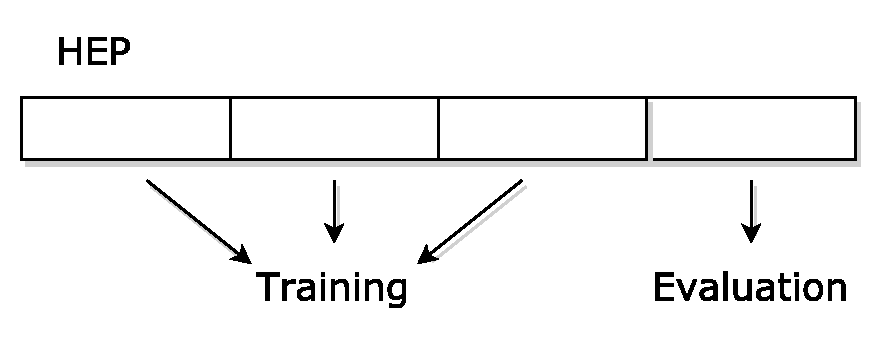
\includegraphics[width=0.28\textwidth]{Figures/CV_HEP.pdf}} & 
\subfloat[CV CORA]{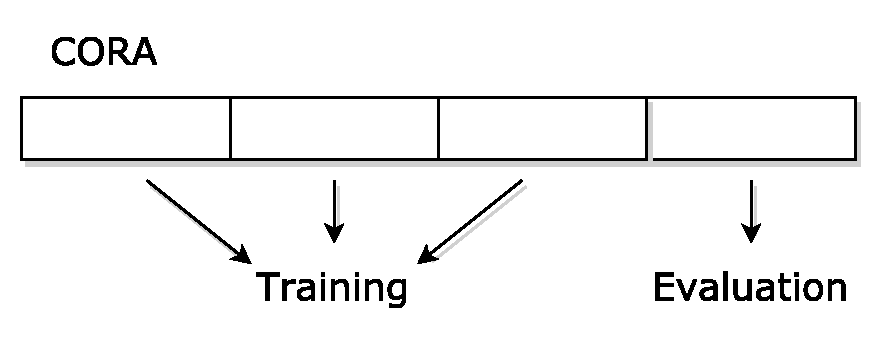
\includegraphics[width=0.28\textwidth]{Figures/CV_CORA.pdf}}\\
\subfloat[CV HEP append CORA]{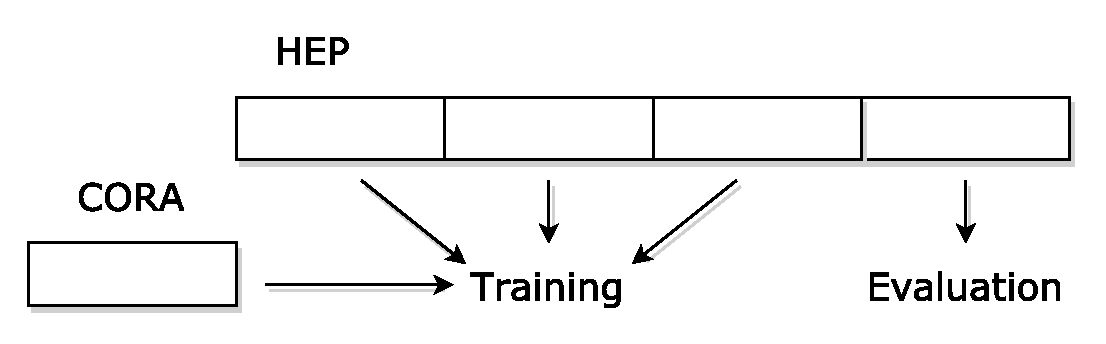
\includegraphics[width=0.35\textwidth]{Figures/CV_HEPappCORA.pdf}} & 
\subfloat[CV CORA append HEP]{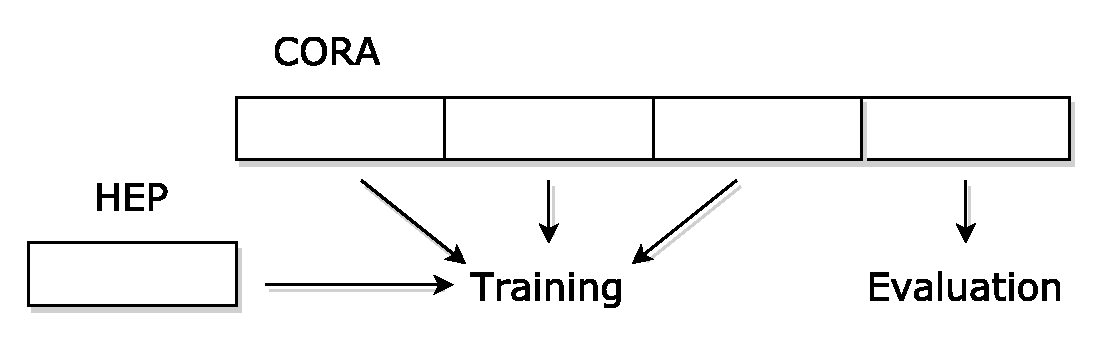
\includegraphics[width=0.35\textwidth]{Figures/CV_CORAappHEP.pdf}}\\ 
% \multicolumn{2}{c}{\subfloat[CV HEP + CORA]{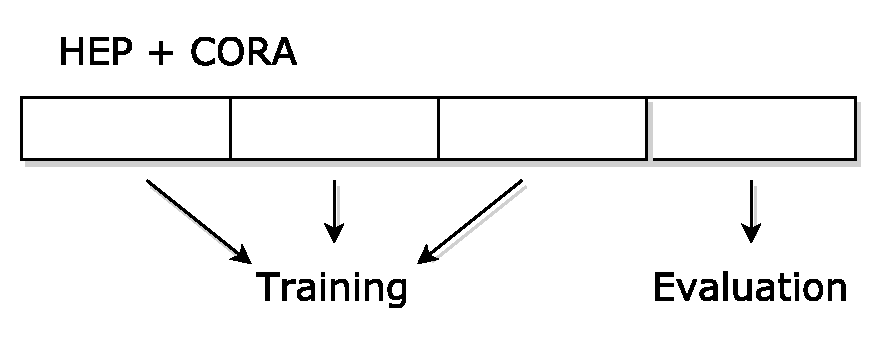
\includegraphics[width=0.36\textwidth]{Figures/CV_HEP+CORA.pdf}}} \\
\end{tabular}
\caption{Cross-validation configurations used in experiments.}
\end{figure}
\end{frame}

%------------------------------------------------

\begin{frame}
\frametitle{Header Model (Subsampling CORA dataset)}
\begin{figure}[h]
\center
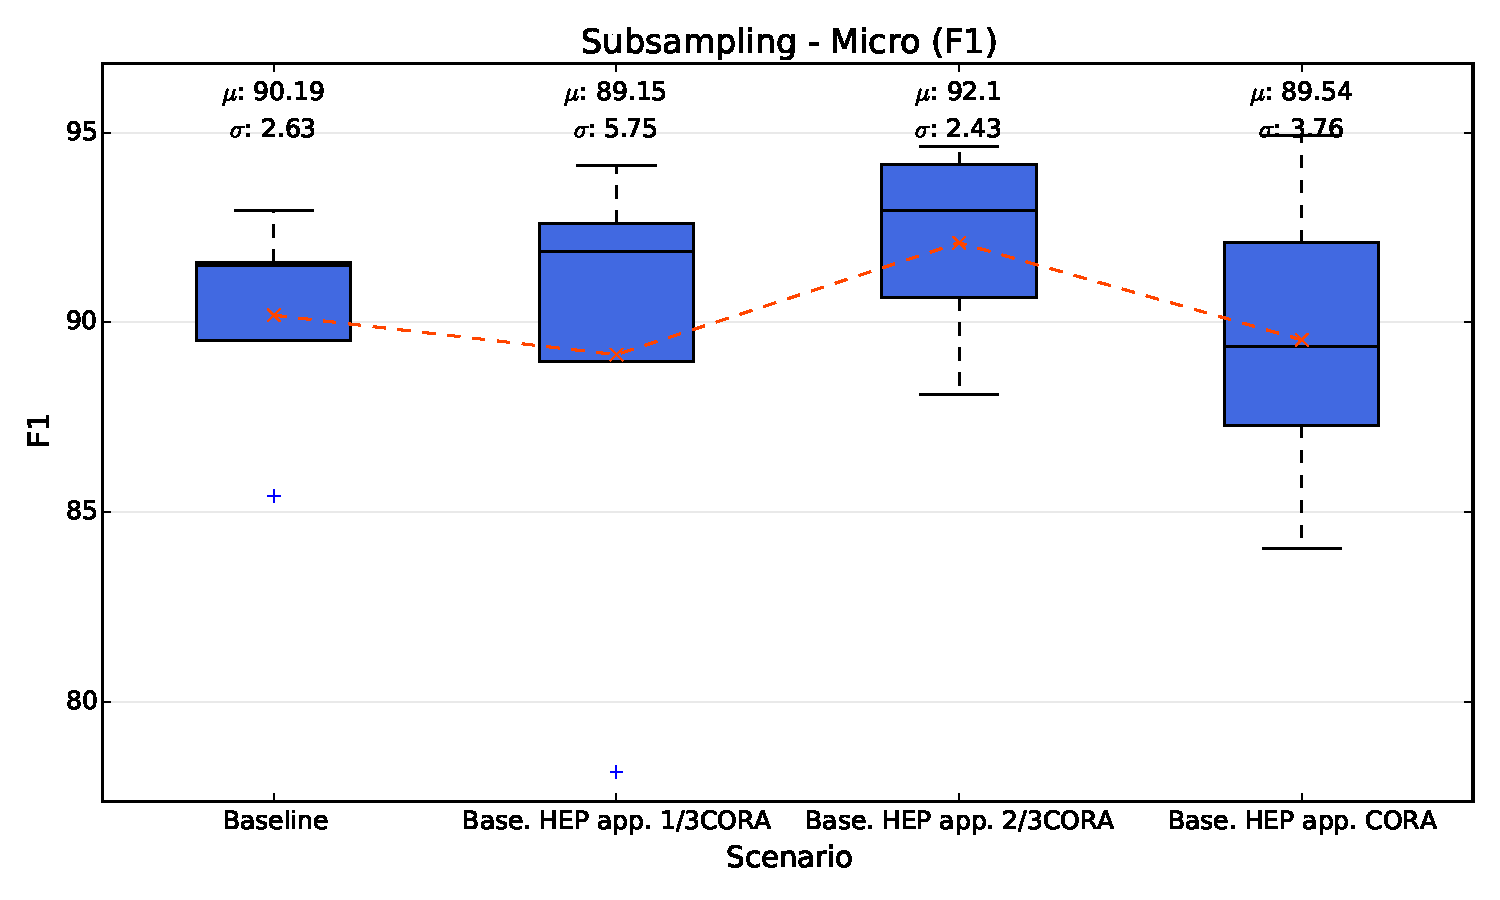
\includegraphics[width=4in]{Figures/micro_subsampling.pdf}
\caption{Appending subsamples of CORA dataset in baseline evaluation.}
\end{figure}
\end{frame}

%------------------------------------------------

\begin{frame}
\frametitle{Header Model (Best Features)}
\begin{figure}[h]
\center
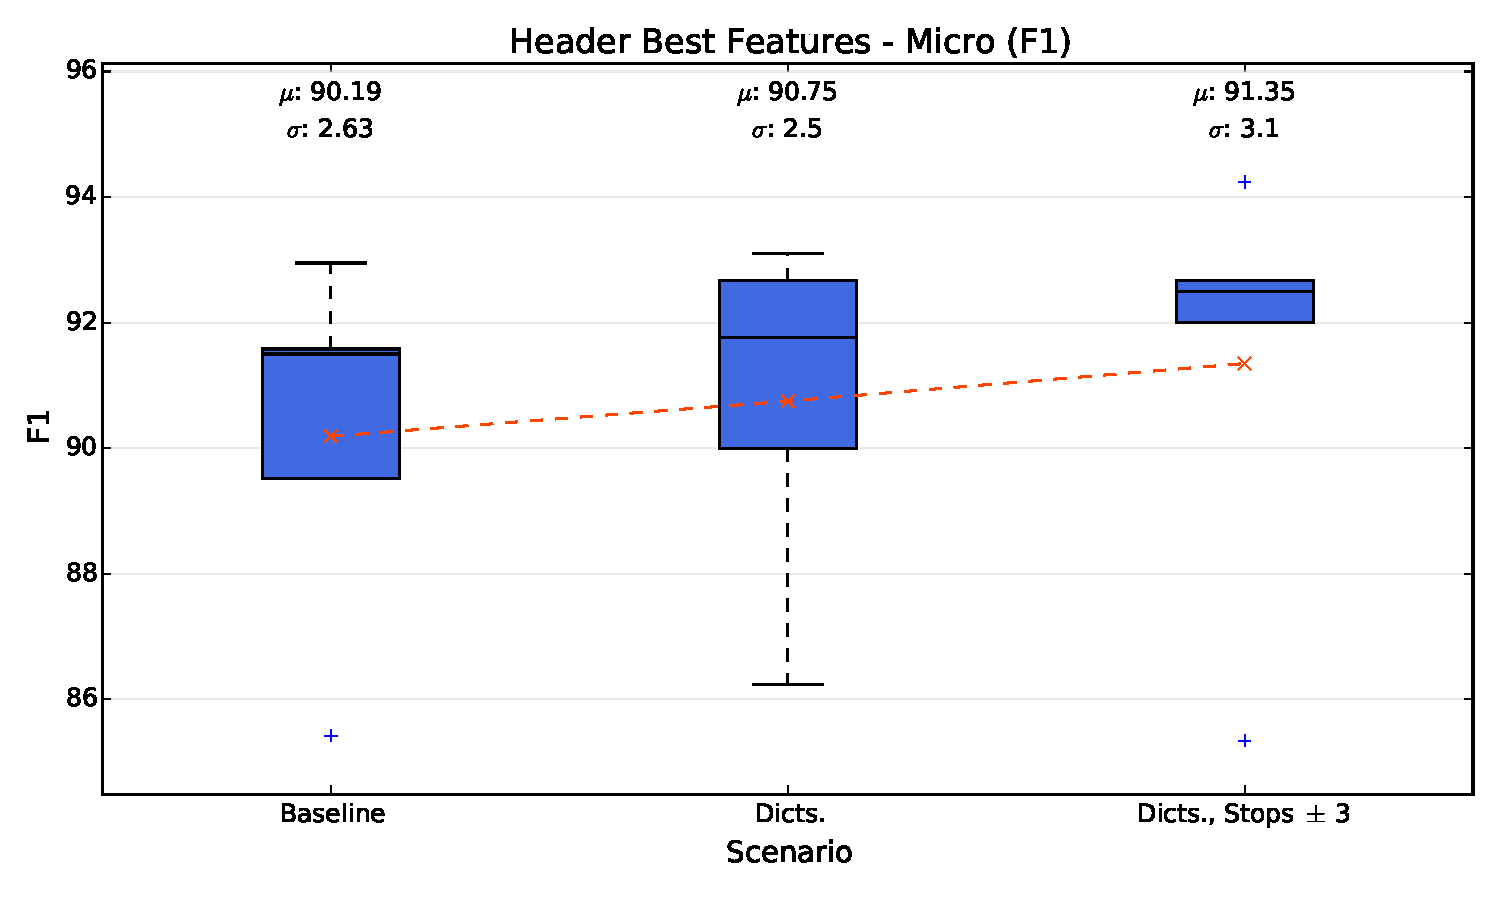
\includegraphics[width=4in]{Figures/micro_header.pdf}
\caption{Best features for header model.}
\end{figure}
\end{frame}

%------------------------------------------------

\begin{frame}
\frametitle{Segmentation Model (Best Features)}
\begin{figure}[h]
\center
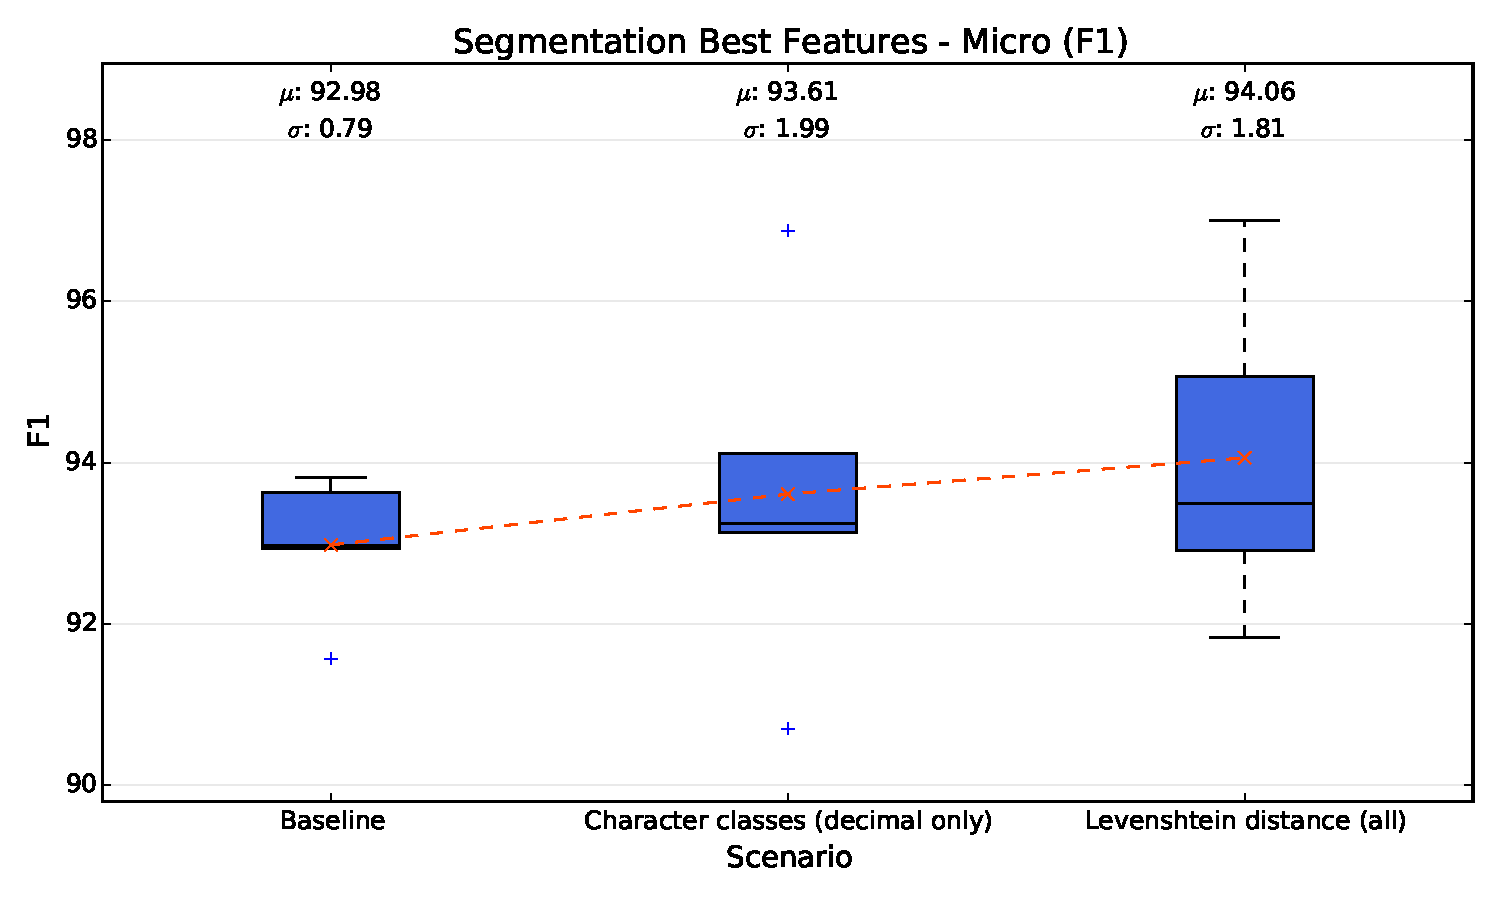
\includegraphics[width=4in]{Figures/micro_segmentation.pdf}
\caption{Best features for segmentation model.}
\end{figure}
\end{frame}

%------------------------------------------------

\begin{frame}
\frametitle{Segmentation Model (Header Field)}
\begin{figure}[h]
\center
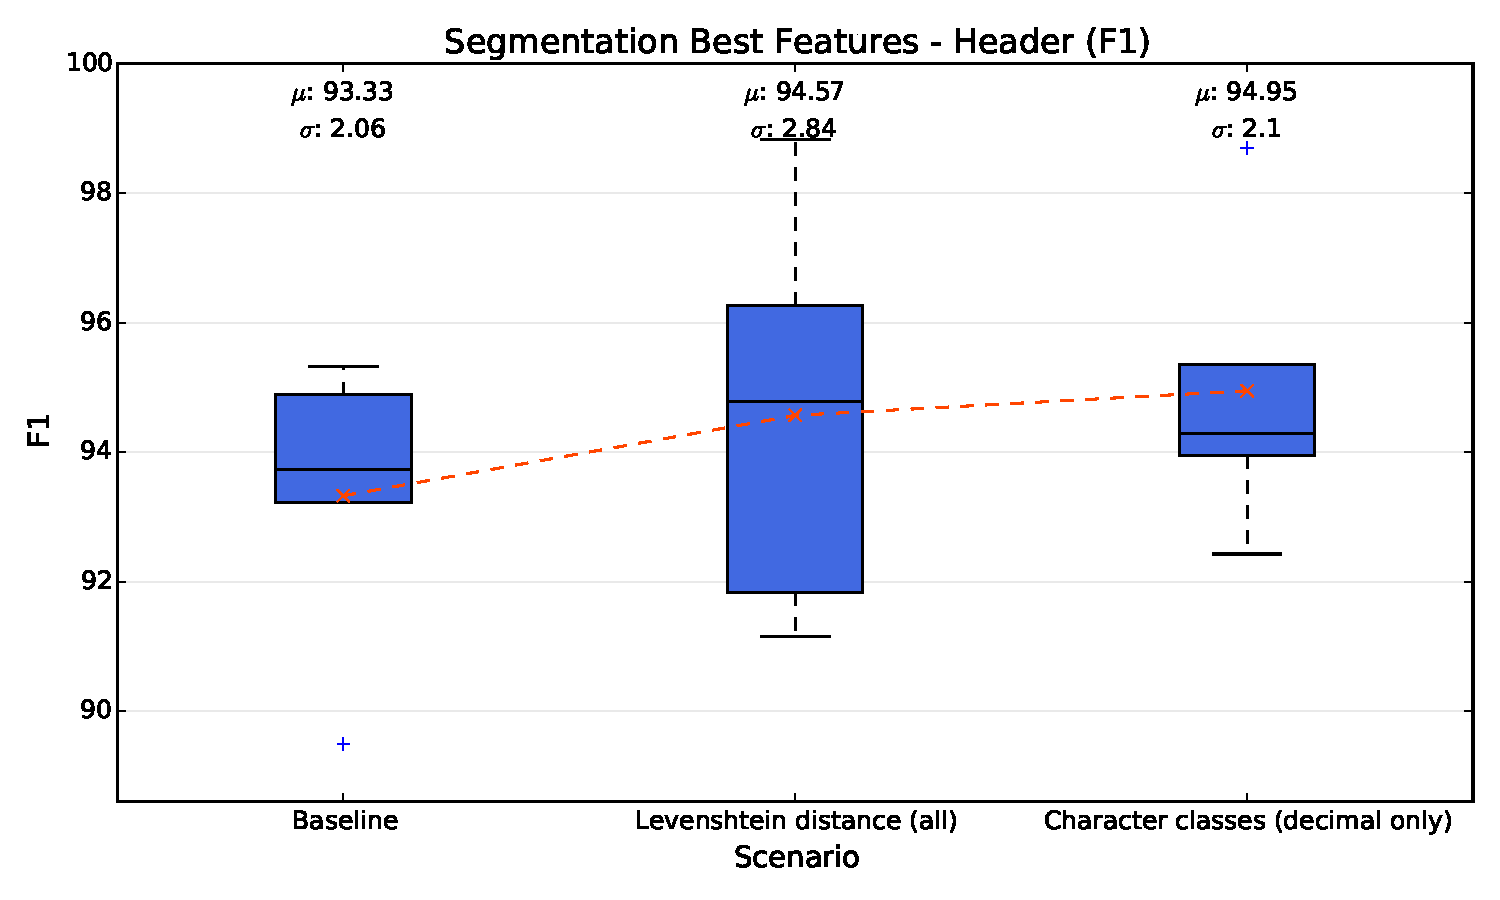
\includegraphics[width=4in]{Figures/header.pdf}
\caption{Best features for segmentation model <header> field.}
\end{figure}
\end{frame}

%------------------------------------------------

\begin{frame}
\frametitle{Segmentation Model (References Field)}
\begin{figure}[h]
\center
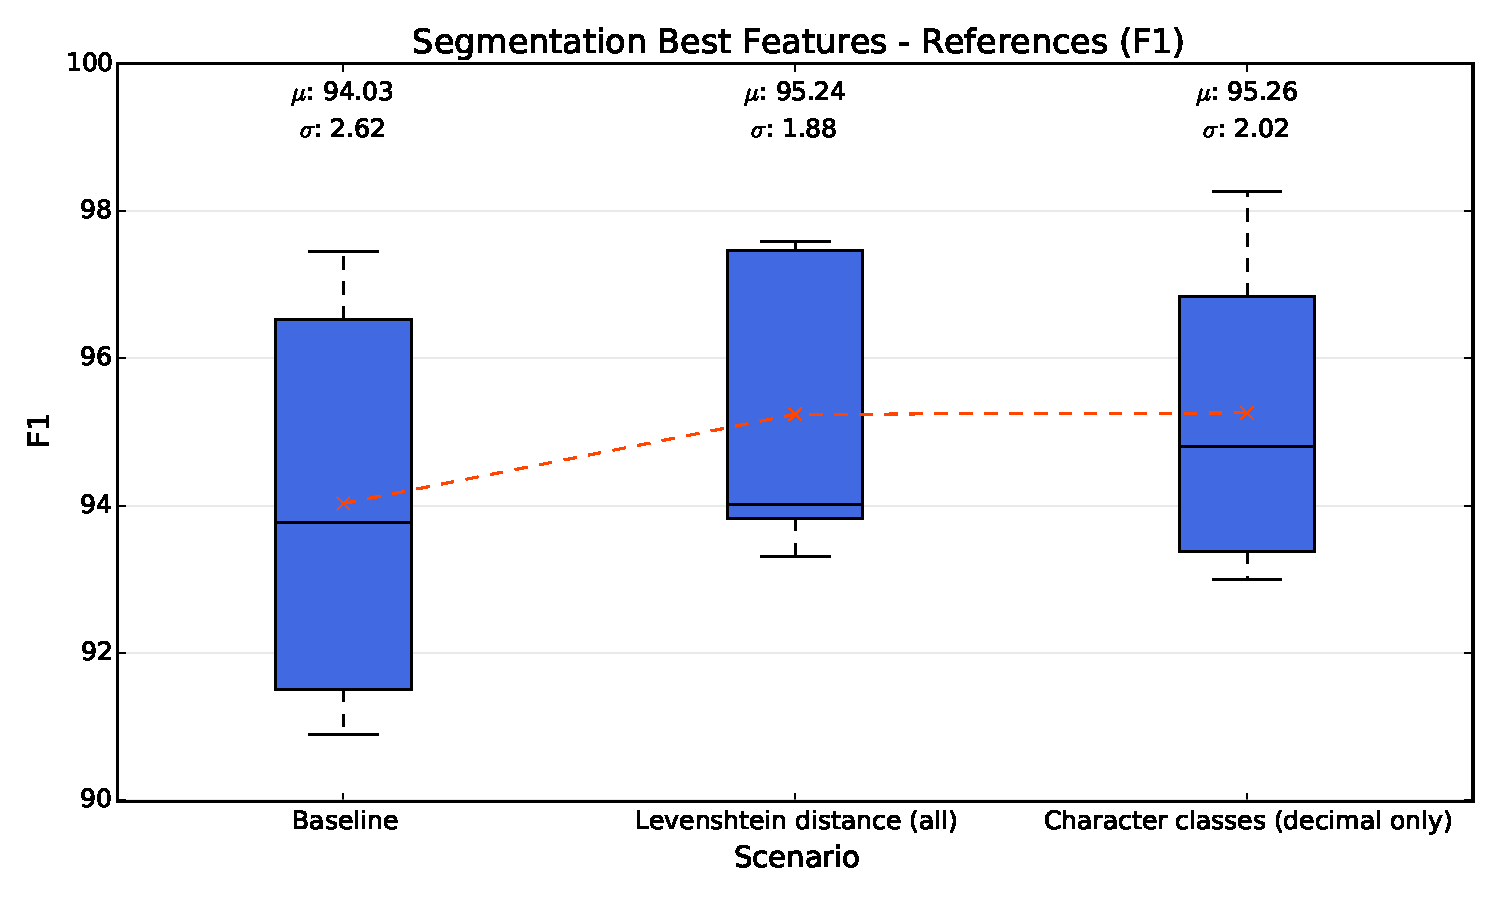
\includegraphics[width=4in]{Figures/references.pdf}
\caption{Best features for segmentation model <references> field.}
\end{figure}
\end{frame}

%------------------------------------------------

\begin{frame}
\frametitle{Segmentation Model (Baseline Confusion Matrix)}
\begin{figure}[h]
\center
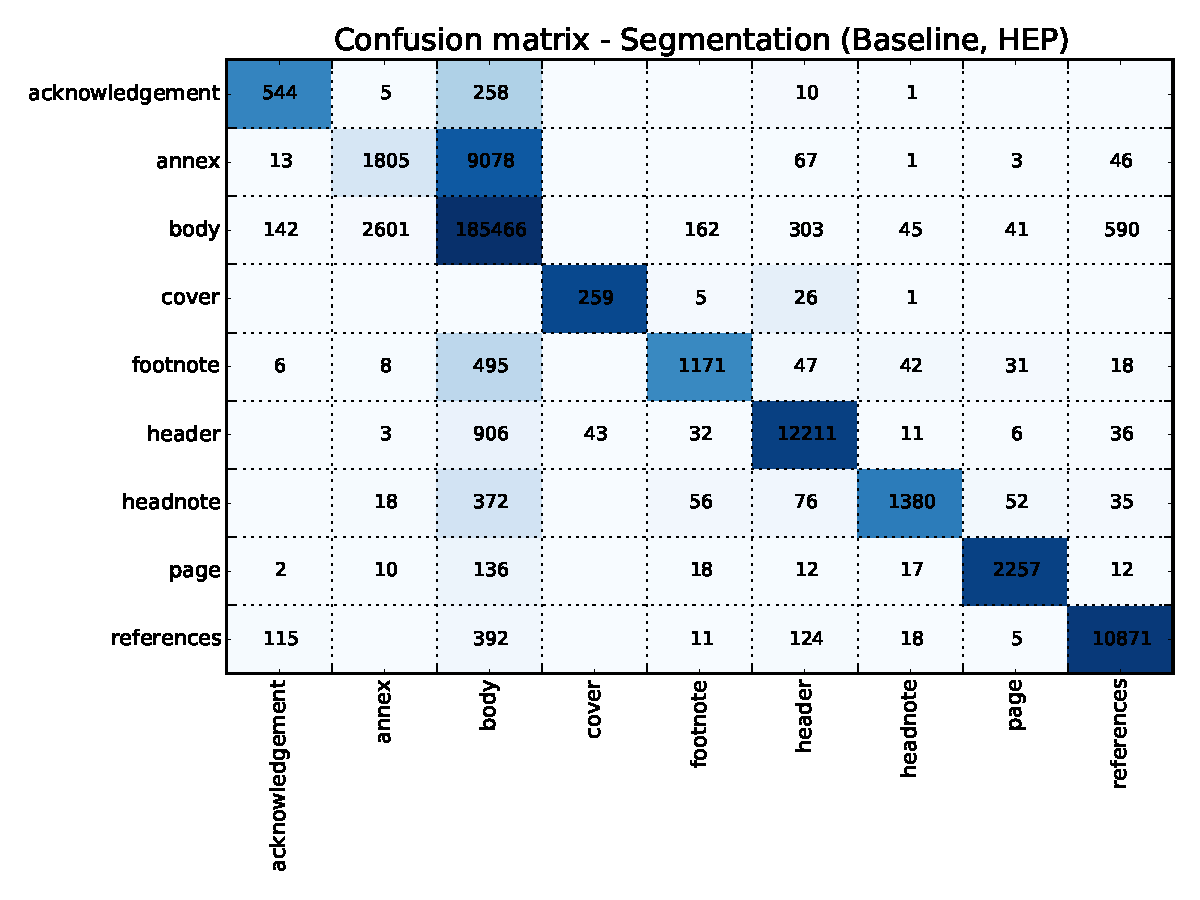
\includegraphics[width=4in]{Figures/baseline_confusion_segmentation.pdf}
\caption{Baseline confusion matrix for segmentation model.}
\end{figure}
\end{frame}

%------------------------------------------------

\begin{frame}
\frametitle{Segmentation Model (Character Class Confusion Matrix)}
\begin{figure}[h]
\center
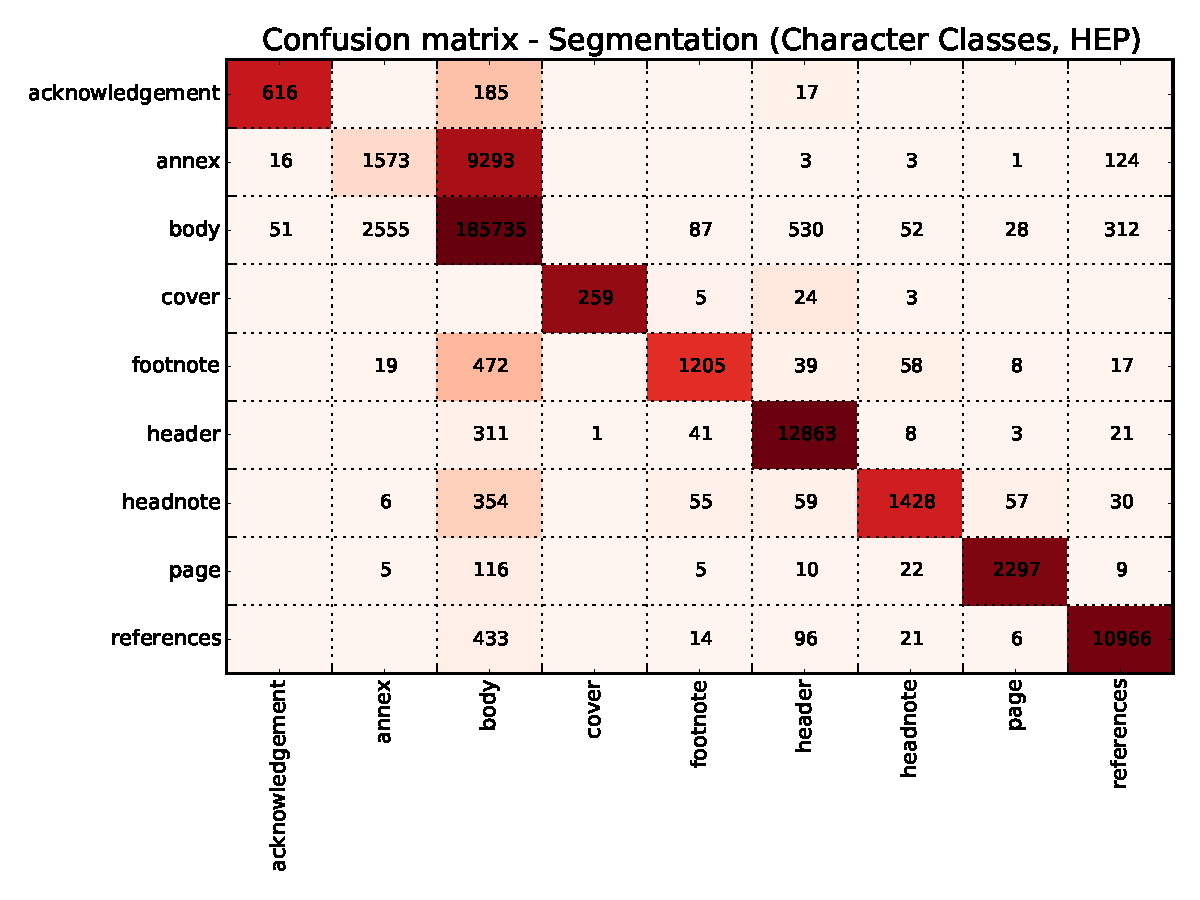
\includegraphics[width=4in]{Figures/classes_confusion_segmentation.pdf}
\caption{Confusion matrix for segmentation model with character classes.}
\end{figure}
\end{frame}

%------------------------------------------------

\section{Conclusions}

%------------------------------------------------

\begin{frame}[noframenumbering]{Outline}
\tableofcontents[currentsection, currentsubsection]
\end{frame}

%------------------------------------------------

\begin{frame}
\frametitle{Conclusions}
\begin{itemize}
\item Qualitative difference between HEP and general papers demonstrated (through inspection, subsampling).
\item Valuable new datasets produced.
\item Successful features offered a dimensionality reduction: dictionaries ($12\%$ error reduction), character classes ($24\%$ and $21\%$ on <header> and <references> classifications).
\end{itemize}
\end{frame}

%------------------------------------------------

\bibliographystyle{ieeetr} % Use the "unsrtnat" BibTeX style for formatting the Bibliography
\bibliography{Bibliography} % The references (bibliography) information are stored in the file named "Bibliography.bib"

\end{document} 